\chapter{Output modules}
\label{chap:Output}

\section{Analogie output}

\begin{figure}[h!]
    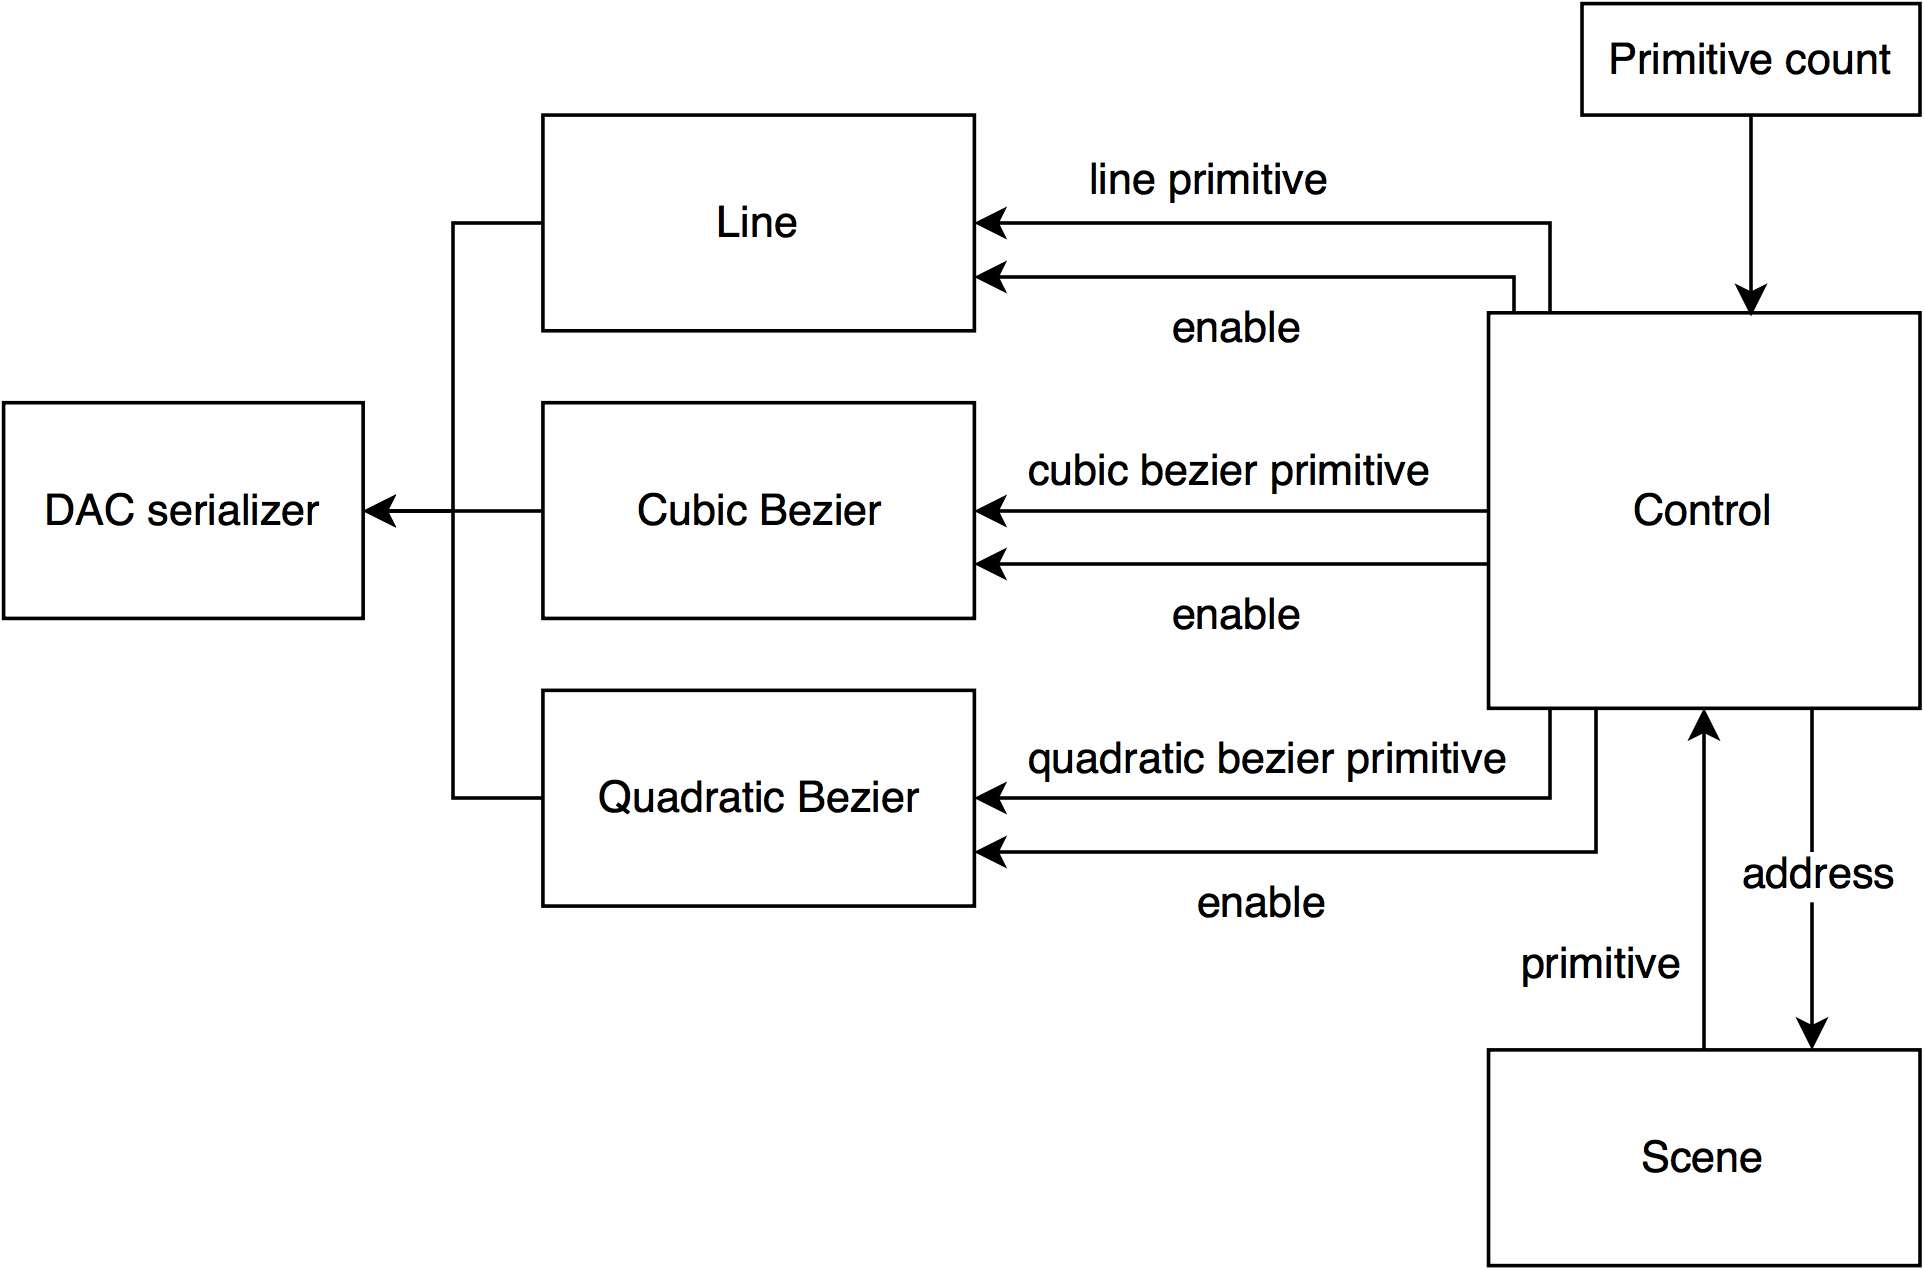
\includegraphics[width=\linewidth]{images/dac-output.png}
    \caption{RTL sketch of the \vthreek DAC output module.}
    \label{fig:dac-output}
\end{figure}

The primary output of the processor is the analogue output.
This output is driven by two DACs that converts digital data from the FPGA to voltages that represents x and y coordinates.
The DACs used are 16-bit which results in an effective resolution of 65536 by 65536 without taking into account the noise on the output voltage.
These DACs have a serial interface and needs 3 signals each to operate; data, clock, and a sync signal.
In order to set an output value on a DAC the sync signal needs to be pulled from high to low then it needs 8 control bits followed by 16 data bits.
After this, the sync signal need to be pulled high again in order to set the output value.
The sync signal can be pulled high before this in order to abort the operation.
Clock and sync signal are shared between the DACs in this system in order to make them change their output synchronously.

The maximum clock frequency of the DACs is 30MHz. 
Since it needs to clock on 24 values per output change as well as the sync signal toggle the effective output maximum will be 30MHz/25=1.2MHz.
However in the implementation the DACs were unstable if clocked any faster than 20MHz which limits the output rate to around 800KHz.

\subsection{Operation}

The output module send an address to the scene memory and gets a primitive back.
There is also another input that keeps track of the number of primitives so the module can restart without reading unused primitives.
It then decodes the primitive and forwards it to the appropriate module or reads a new primitive if no primitive was found and forwards the output of this module to the DAC serializer.
The respective serializer will then calculate a fixed number of points along the line or curve.
A fixed number of points was chosen because there was no time to implement any functionality for calculating the lengths of lines or curves accurately.
This will result in shorter lines and curves appearing brighter on the oscilloscope.

The actual calculation of the points is done by using the equations described in section \ref{sec:bezier}.
However since there was no floating point unit, a number between 0 and 1023 was used instead of a number between 0 and 1, that was then left shifted by 5.
t then becomes \(t = i \ll 5\) (\(0 \geq i < 1024\)). 
After every multiplication the result is then right shifted by 15.
This results in a limit of 1024 different points for a given primitive.

The calculation for points for every type of primitive is largely the same, however the different number of points per primitive needs to multiplied by a different factor. 
The equation for these can be found in section \ref{sec:bezier}

\section{Raster output}

This output uses HDMI to output a rasterized image of the internal vector representation.
In order to generate the rasterized frame the x and y output from the vector output described in the previous section would be written into a frame-buffer.
This buffer can then be scaled to the desired output resolution and run through TMDS encoder and output via HDMI.